\chapter{Logik}

\section{Projektstruktur}

Das Projekt lässt sich in mehrere Teilmodule (Packages) aufgliedern. Gemäß dem objektorientieren Programmieren werden Klassen, die einen logischen Zusammenhang besitzen, in ein Package zusammengefasst.

\begin{figure}[!ht]
\centering
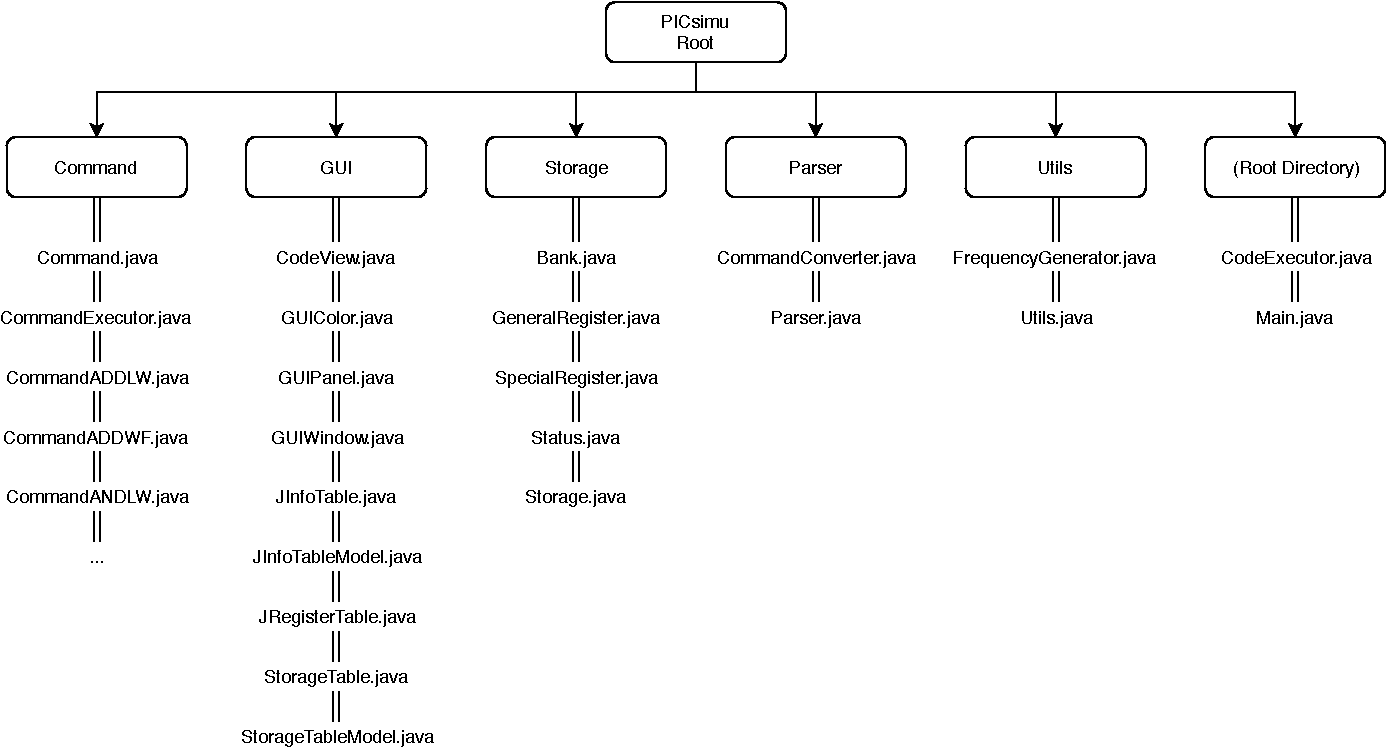
\includegraphics[width=\textwidth]{img/PICsimu-tree.pdf}
\caption{Projektstruktur-Baum}
\label{project-tree}
\end{figure}

\noindent In diesem Projekt gibt es nachfolgende Packages; es werden die darin wichtigsten Klassen erklärt.

\begin{description}
\item[Command]{Dieses Package beinhaltet die Klassen zu sämtlichen Assemblerbefehlen - von \textit{ADDLW} bis \textit{XORWF}. Zudem gibt es die Superklasse \textit{CommandExecutor} mit Methoden, welche das Status-Register nach einer Rechenoperation beeinflussen. In der Enumeration \textit{Command} werden alle Befehle aufgelistet - inklusive Befehlscode, Argumentmaske, Anzahl Quarztakte sowie die \enquote{Status Affected Bits}.}
\item[GUI]{Dieses Package beinhaltet die Klassen zur grafischen Oberfläche - dem Frontend. \textbf{TO BE CONTINUED...}}
\item[Storage]{Dieses Package beinhaltet die Klassen zum (Register-) Speicher sowie zur Bankumschaltung. Die Enumeration \textit{SpecialRegister} beinhaltet eine Auflistung der Spezialregister (z.B. Status-Register) mit deren Speicheradressen und Standardbelegung. In der Klasse \textit{Storage} wird der Speicher (inklusive EEPROM) des Mikrocontrollers verwaltet.}
\item[Parser]{Dieses Package beinhaltet die Klasses zum Parsing der Programme für den Mikrocontroller. \textbf{TO BE CONTINUED...}}
\item[Utils]{Dieses Package beinhaltet Klassen mit nützlichen (programminternen) Hilfsmethoden sowie einen einstellbaren Frequenzgenerator, der an die Pins von PORTA bzw. PORTB angelegt werden kann.}
\item[(Root Directory)]{Dieses Package ist das Root Verzeichnis der Packages. In diesem liegen alle anderen Packages sowie die Klasse \textit{Main} und \textit{CodeExecutor}. \textbf{TO BE CONTINUED...}}
\end{description}